\documentclass[11pt, a4paper,english,spanish]{article}
\usepackage[spanish]{babel}
\usepackage[utf8]{inputenc}
\usepackage{gensymb}
\parskip = 11 pt
\usepackage[width=18cm, left=1.5cm, top=2.25cm, height= 25cm]{geometry}

\usepackage{amsmath}
\usepackage{algorithm}
\usepackage[noend]{algpseudocode}
\usepackage{amsfonts}
\usepackage{amssymb}
\usepackage{fancyhdr}
\usepackage{lastpage}
\usepackage{caratula}
\usepackage{url}
\usepackage{flafter}
\usepackage{afterpage}
\usepackage{float}
\usepackage{listings}
\usepackage{color}
\usepackage{verbatim}
\definecolor{gray97}{gray}{.97}
\definecolor{gray75}{gray}{.75}
\definecolor{gray45}{gray}{.45}

\algdef{SE}[DOWHILE]{Do}{doWhile}{\algorithmicdo}[1]{\algorithmicwhile\ #1}%
 
\usepackage{listings}
\lstset{ frame=Ltb,
     framerule=0pt,
     aboveskip=0.5cm,
     framextopmargin=3pt,
     framexbottommargin=3pt,
     framexleftmargin=0.4cm,
     framesep=0pt,
     rulesep=.4pt,
     backgroundcolor=\color{gray97},
     rulesepcolor=\color{black},
     %
     stringstyle=\ttfamily,
     showstringspaces = false,
     basicstyle=\small\ttfamily,
     commentstyle=\color{gray45},
     keywordstyle=\bfseries,
     %
     numbers=left,
     numbersep=15pt,
     numberstyle=\tiny,
     numberfirstline = false,
     breaklines=true,
   }


% minimizar fragmentado de listados
\lstnewenvironment{listing}[1][]
   {\lstset{#1}\pagebreak[0]}{\pagebreak[0]}
 
\lstdefinestyle{consola}
   {basicstyle=\scriptsize\bf\ttfamily,
    backgroundcolor=\color{gray75},
   }
 
\lstdefinestyle{C++}
   {language=C++,
   }
 
\newcommand{\real}{\ensuremath{\mathbb{R}}}
\newcommand{\grad}{\hspace{-2mm}$\phantom{a}^{\circ}$}

\pagestyle{fancy}

\title{MotionCapture}

%Estilo para el encabezado
\fancyhead[LO, LE]{Métodos Numéricos}
\fancyhead[RO, RE]{2$^{do.}$ cuatrimestre de 2014}
\fancyhead[CO, CE]{}

\fancyfoot[CO, CE]{P\'agina \thepage\ de \pageref{LastPage}}

\begin{document}
%Estos son los parametros para la caratula
\materia{Métodos Numéricos}
\submateria{Trabajo Pr\'actico Nro. 1}
\titulo{Sanguijuelas}
\fecha{\today}
\integrante{Martin Carreiro}{45/10}{martin301290@gmail.com}
\integrante{Kevin Kujawski}{459/10}{kevinkuja@gmail.com}
\integrante{Juan Manuel Ort\'iz de Z\'arate}{403/10}{jmanuoz@gmail.com}
\maketitle
\newpage

%Pagina de titulo e indice
\thispagestyle{empty}

\tableofcontents

\newpage

\normalsize
\section{Resumen}

Mediante el manejo de matrices se buscará modelar y resolver un problema de la realidad. Cómo la realidad está compuesta de infinitas variables dicha modelización implicará una inevitable discretización. Es decir trabajar con una 
cantidad acotada de variables del problema (sólo las relevantes).

El problema en cuestión es representar un parabrisas al cual se le adhieren sanguijuelas que le producen calor en un radio de las mismas. Queremos evitar que el parabrisas llegue a un punto crítico, que implicaría la destrucción de este. El punto crítico ocurre cuando el punto del centro tienen más de 235${}^o$C. Para evitar que llegue al punto crìtico debemos deshacernos de las sanguijuelas pero no tenemos la energía para destruirlas a todas, por lo que tenemos que achicar la cantidad de sanguijuelas a eliminar de forma tal que el parabrisas no se rompa.

La modelización del mismo no es trivial. Es más, podría decirse que este proceso es mucho más complejo y costoso que la solución en sí. ¿Por qué? porque la creación de la matriz que represente al parabrisas y el cálculo de las temperaturas en cada punto, si no se usa un buen método, podría llegar a demorar mucho tiempo. 

Por esto es que a lo largo del TP haremos mucho foco en como representar en forma de matriz el parabrisas, como este puede llegar a tener propiedades que utilizaremos para ahorrar el espacio ocupado. Una vez que tengamos esto, necesitamos saber si realmente estámos bajo un punto crítico. Esto estará determinado por la posición central  de la matriz que discretiza el parabrisas $(altura/2,ancho/2)$ (donde altura y ancho son las cantidad de celdas correspondientes) y su temperatura (si es mayor o menor a 235${}^o$C) para saber así si necesitamos deshacernos de las sanguijuelas para poder seguir navegando.

Una vez que tengamos esto plantearemos casos de test interesantes para analizar el tiempo de decisión de una situación de peligro y que el método elegido para deshacernos de las sanguijuelas nos minimiza la cantidad a destruir.

\textit{Se acompaña el informe con el código en C++ y los archivos .in que utilizamos para la experimentación}



\newpage
\section{Introducci\'on te\'orica}

Dado que la modelización utlizada para este problema es un sistema de ecuaciones y que en base a algunos datos que nos dan (posición de las saniguijuelas, dimensiones y temperaturas de los bordes) tenemos que calcular los valores de muchas celdas, lo que hay que resolver es un sistema de ecuaciones. 
Lo primero que se nos viene a la mente cuando tenemos esto es el método de eliminación gaussiano. Este transforma la matriz de coeficientes en una matriz triangular superior y luego mediante back substitution 
se pueden obtener todos sus valores. Si bien este método no funciona siempre veremos que para nuestro caso puede otorgarnos soluciones aceptables.

Veamos ahora más en detalle como funciona cada uno de estos algoritmos.

\subsection{Algoritmo de eliminación gaussiana}

Este algoritmo consisnte en restar multiplos de filas entre sí, comenzando desde la primera, con el objetivo de lograr todos ceros por debajo de la diagonal y numeros disintos de cero en la diagonal, 
es decir una matriz triangular superior. En el caso que me quedase un 0 en la diagonal el algoritmo comprende la opción de pivoteo (mas adelante demostraremos que en realidad no necesitamos) que consiste en intercambiar 
filas entre sí para que esto no suceda.

Veamos ahora algún ejemplo concreto con la siguiente matriz de $3 \times 3$:

\[ \left( \begin{array}{ccc}
4 & 8 & 9 \\
1 & 5 & 2 \\
2 & 3 & 1 \end{array} \right)\] 

Hago 

\emph{F2 = F2 - 1/4 (F1) y F3 = F3 - 1/2 (F1)} 
\[ \left( \begin{array}{ccc}
4 & 8 & 12 \\
0 & 3 & -1 \\
0 & -1 & -5 \end{array} \right)\] 

y ahora

\emph{F3 = F3 - -1/3 (F2) } 
\[ \left( \begin{array}{ccc}
4 & 8 & 12 \\
0 & 3 & -1 \\
0 & 0 & -31/3 \end{array} \right)\] 

Si entendemos la matriz original como un sistema de ecuaciones con 3 variables igualadas a distintos resultados, como podemos ver a continuación:

\[ \left( \begin{array}{ccc}
4x & 8y & 9z \\
1x & 5y & 2z \\
2x & 3y & 1z \end{array} \right)\] 

Con esta nueva matriz triangulada podríamos calcular facilmente el valor de cada variable ya que de la última ecuación podemos despejar facilmente el valor de Z, reemplazarlo en las otras ecuaciones y así calcular las otras variables.



Por último cabe destacar que la complejidad computacional de esta trinagulación es de O($n^3$). Lo cual puede llegar a un cálculo sumamente extenso si nuestro n es considerablemente importante. Por esto es que decidimos pensar un poco mas la situación y encontrarle la vuelta para resolver en un tiempo razonable.

\subsection{Matriz banda}

Matriz banda es un caso especial de las matrices que ocurre cuando estas concentran toda su información cerca de la diagonal, más especificamente, la matriz tiene en su mayoría elementos nulos y los que no son nulos se concentrar a izquierda y derecha de la diagonal de la matriz, siendo el máximo de estas distancias la que determinaran el ancho de la banda con que se denomine a la matriz y buscandose que las mismas sean relativamente pequeñas en comparación del ancho de la matriz. Por ejemplo, si a lo sumo tiene $p$ elementos no nulos a la izquierda y $q$ a la derecha, esta matriz tendrá una banda de $p+q+1$. Hay casos particulares para denominar estas matrices, por ejemplo, cuando $p = q = 0$ esta se denomina diagonal, y en caso de $p = q = 1$  es una tridiagonal.
La ventaja principal que proporcina este tipo de matriz es la optimización a la hora de su almacenamiento, ya que como la mayoría de los elementos son nulos y los no nulos tiene un ancho fijo, es posible guardarlos en una matriz mucho menor con solo el tamaño de la banda como ancho, ahorrando gran cantidad de memoria.

Aca podemos ver un ejemplo de una matriz banda:

\emph{ Matriz banda tridiagonal } 
\[ \left( \begin{array}{ccccccc}
d & q & 0 & 0 & 0 & 0 \\
p & d & q & 0 & 0 & 0 \\
0 & p & d & q & 0 & 0 \\
0 & 0 & p & d & q & 0 \\
0 & 0 & 0 & p & d & q \\
0 & 0 & 0 & 0 & p & d \end{array} 
\right)\] 

En el ejemplo se puede ver como se forma la banda sobre la diagonal, con la mayoría de elementos nulos fuera de la misma. Por lo tanto para ahorrar espacio se puede optimizar su almacenamiento de la siguiente forma:

\emph{ Almacenamiento sólo de la banda de la matriz original } 
\[ \left( \begin{array}{ccc}
0 & d & q \\
p & d & q \\
p & d & q \\
p & d & q \\
p & d & q \\
p & d & 0 \end{array} 
\right)\] 


En la sección Desarrollo mostraremos como aprovecharemos las ventajas de este tipo de estructura para resolver el problema planteado de una forma más eficiente. 






\newpage
\section{Desarrollo}

\subsection{Eliminación Gaussiana}
 A modo de comparación recreamos el clásico método de resolución de Eliminación Gaussiana que consta de la eliminación progresiva de variables en el sistema de ecuaciones, hasta tener sólo una ecuación con una incógnita. Una vez resuelta esta, se procede por sustitución regresiva hasta obtener los valores de todas las variables.

\begin{verbatim}
Class Windshield{
    resolveByGaussianElimination(){
         gaussianElimination();
         backSubstitution();
    } 
    gaussianElimination(){
        for rows k already been reduced
            iMax = findPivot();
            Swap rows k and imax;
            Force 0’s in column A[k+1..n-1][k];
    }
    backSubstitution(){
        for row from last to first:
            calculateFromNextOneExceptForLast()
    }
}
\end{verbatim}

\subsection{Matriz Banda}

En la sección anterior presentamos una forma de resolver nuestro problema representando el parabrisas como un sistema de ecuaciones y aplicando Eliminación Gaussiana. En este sección propondremos una optimización a esto, pero para esto primero necesitamos ver con qué cosas estamos tratando y para eso veamos el siguiente ejemplo:

En este caso es un parabrisas de 6x6 granulado en 1 y una sanguijuela de radio 1 con temperatura de 500 en la primera posición.

El parabrisas se vería representado asi (hay que tener en cuenta que en realidad hay que espejarlo horizontalmente ya que para nosotros el eje de coordenadas se encuentra arriba a la izquierda):

\begin{figure}[htb]
\begin{center}
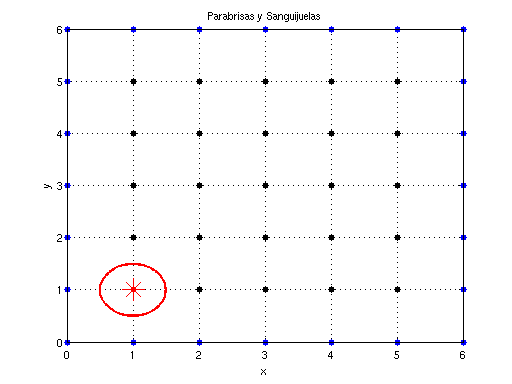
\includegraphics[scale=0.40]{imagenes/matrizbandaej_instancia.png} 
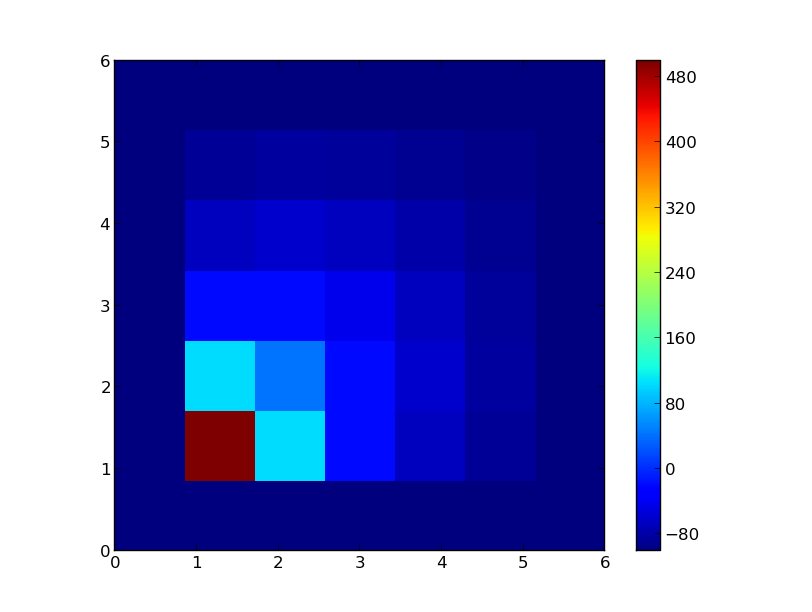
\includegraphics[scale=0.40]{imagenes/matrizbandaej_temp.png} 
\end{center}
\end{figure}

\newpage

Planteando el parabrisas como un sistema de ecuaciones sin tener en cuenta que es banda y por consiguiente sin realizar ninguna optimización al respecto, la matriz quedaría como el siguiente gráfico, donde en cada fila se representa todo el parabrisas como un vector $'aplanado'$ pero hace referencia a una en particular. Por lo tanto la diagonal de la matriz representa al coeficiente de esa posición en el parabrisas.
En base a lo que explicamos anteriormente y como la temperatura de cada celda vacía es el promedio de las 4 contiguas, al plantear la ecuación: 
\[
t_{ij} = (t_{i+1 j} + t_{i j+1} + t_{i-1 j} + t_{i j-1}) / 4
\]

\[
4 t_{ij} = t_{i+1 j} + t_{i j+1} + t_{i-1 j} + t_{i j-1}
\]

\[
4 t_{ij} - t_{i+1 j} - t_{i j+1} - t_{i-1 j} - t_{i j-1}  = 0
\]

Nos queda que los coeficientes de la celda actual es 4 y de las contiguas un -1, igualando todo a cero.
Por lo tanto en cada fila de la matriz calculamos la posición que deberia queda cada celda contigua en la matriz aplanada, quedando el sistema de ecuaciones de la siguiente forma: \\
(donde los espacios vacios representan blancos)
\begin{figure}
\begin{center}
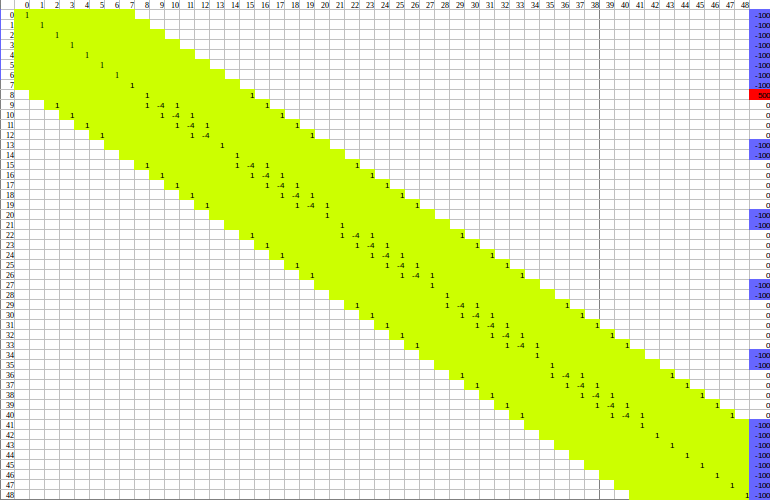
\includegraphics[scale=0.60]{imagenes/matrizej.png} 
\caption{Matriz de ecuaciones del ejemplo} 
\end{center}
\end{figure}


\newpage

Analizando la matriz del sistema de ecuaciones que se genera a partir de la representación del Parabrisas observamos que presenta las caracteristicas de un tipo de matriz llamada $``banda"$, la cual se distingue por tener todas las celdas en 0 salvo en la diagonal ensanchada, es decir, que $p$ celdas a la izquierda y $q$ a la derecha de la diagonal a lo sumo tienen algunos o todos los valores distintos de 0. 
Este es un hecho importante ya que las matrices banda tienen caracteristicas especiales de las cuales es posible la optimización temporal y espacial para resolver el sistema de ecuaciones con eliminación gausseana.

\subsubsection{Optimización}

El problema de representar la matriz original es que la mayoría de los valores son 0 y solo importan los elementos de la banda de la matriz, por lo tanto una forma de optimizar espacialmente es solo guardar la banda, con lo que se logra reducir considerablemente el espacio en esta representación, ya que suponiendo que se tiene un parabrisas de $n$ filas y $m$ columnas, el tamaño de la matriz original sería de $(n*m)^2$, mientras que con la optimización de matriz banda queda de tamaño $(n*m)*(2*m+1) \approx (n*m^2)$ .

El método para construir la representación optimizada de la matriz banda es simple, se guarda la banda en una matriz pero rotandola de forma que quede vertical, quedando en el centro los elementos de la diagonal dependiendo de lo que haya en esa posición, ya que en el caso de que sea vacía esta deberá tener coeficientes de las posiciones adyacentes.
Aúnque uno podría pensar que ya que solo hay 4 elementos no nulos máximo en cada fila se podria optimizar guardando esos 4 coeficientes, pero debido a que luego se le aplicará el método de Back Substitution de la Eliminación Gausseana como método para resolver el sistema, esto hará que se generen valores no nulos dentro de la banda, por lo tanto el tamaño de esta matriz deberá ser lo suficiente como para poder trabajar sobre él y almacenar los valores parciales.

El algoritmo consta de dos etapas, la construcción de la matriz que representara la banda y la resolución del problema utilizando la misma.

\paragraph{Construcción de la matriz banda}
\begin{verbatim}

por cada posición del parabrisas //O(N*M)
       pos = fila posicion + columna posicion * ancho;
		
              si en esa posición hay una SANGUIJUELA:
			
                    bandMatrix[pos][ancho] = 1;
                    resultados[pos] = ts;
		
              si esa posición es borde FRIO:
                    
                    bandMatrix[pos][ancho] = 1;
                    resultados[pos] = -100;


              en caso de que esa posición sea VACIA:
                    bandMatrix[pos][ancho] = -4;
                    resultados[pos] = 0;              
                    bandMatrix[pos][ancho-1] = 1;
                    bandMatrix[pos][0] = 1;
                    bandMatrix[pos][ancho+1] = 1;
                    bandMatrix[pos][ancho*2] = 1;
		

\end{verbatim}

\paragraph{Resolución del sistema}

\begin{verbatim}

//PRIMERO LA HAGO TRIANGULAR SUPERIOR
PARA CADA FILA DE LA BANDA, DE ARRIBA A ABAJO
		
   SI NO ES VACIO SE QUE ABAJO HAY TODO CERO, CONTINUO
   SI ES VACIA DIAGONALIZO:
        
         centro = bandMatrix[i][n];
         actual = bandMatrix[i+h][n-h];
         multiplicador = actual / centro;
		
         fila[i+h] - fila[i];

         resultado[i+h] -= resultado[i] * multiplicador;
   

    //BACK SUBSTITUTION
    PARA CADA FILA DE LA BANDA, DE ABAJO A ARRIBA
        fila = i / n;
        for( int h = 1; h <= n; h++){ // COMO ES BANDA ME FIJO SI EN LA DIAGONAL IZQ INF HAY DISTINTO DE 0 PARA PIVOTEAR
           
             centro = bandMatrix[i][n];
             actual = bandMatrix[i-h][n+h];
           
             multiplicador = actual / centro;
		
             fila[i-h] - fila[i];
             resultado[i-h] -= resultado[i]* multiplicador;
                
             lleno el parabrisas con las temperaturas actuales
\end{verbatim}


\subsubsection{Ejemplo}

Aca podemos ver un ejemplo para ver como funciona lo explicado en esta sección.


Pero en vez de eso al optimizar la matriz banda se genera esta matriz:

\begin{figure}
\begin{center}
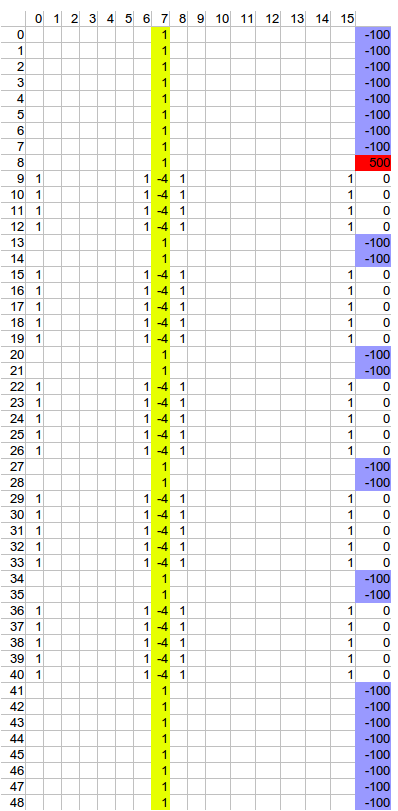
\includegraphics[scale=0.70]{imagenes/matrizbandaej.png} 
\caption{Matriz banda del ejemplo} 
\end{center}
\end{figure}




\section{Eliminar sanguijuelas}

La resolución del problema de evitar el punto crítico en el centro del parabrisas consiste en la eliminación de sanguijuelas. Suponiendo la existencia de $n$ sanguijuelas, los cantidad de subconjuntos a probar son $2^n$. Es un número que crece rápidamente y si bien se puede resolver por fuerza bruta (ayudados por Backtracking y derivados), suponemos que encontrar el mínimo tiene un orden exponencial en la cantidad de sanguijuelas.

Finalmente, planteamos dos tipos de solución a modo de comparación. Estos serán detallados más adelante. Ambas son heurísticas por lo mencionado anteriormente.

\subsection{Punto Crítico}
En un parabrisas real el punto crítico se determina por el punto exacto del medio del parabrisas, en la posición (largo/2, ancho/2), pero en nuestra estructura de datos que representa al parabrisas esta puede no llegar a tener un punto exacto dependiendo de la discretización que tenga el mismo. Por lo tanto tenemos dos casos, el caso $"$trivial$"$ es hay un punto exacto donde cae el punto crítico en el parabrisas, en ese caso elegimos ese. En el caso contrario, cuando tomamos la mitad del largo y ancho del parabrisas para elegir el punto crítico este no sera un número entero, por lo tanto redondearemos para abajo y el punto crítico que consideraremos se priorizara teniendo el cuenta el que esta más arriba a la izquierda.

\subsection{Solución Greedy}
Esta solución consiste en ir seleccionando las sanguijuelas más cercanas al punto medio hasta que el punto central esté por debajo de 235 Cº. Al no ser una solución exacta es posible que eliminar la más cercana al centro no pertenezca a la mejor solución, pero es intuitivo suponer que la sanguijuela que más cause calor al punto medio esté cerca del mismo. \\
Lo primero que se realiza es ordenar las sanguijuelas según su distancia al centro. Para esto utilizamos la función $sort()$ de C++ que utiliza como comparador el valor pre-calculado de distancia al centro. El orden de esta parte es $O(n.log(n))$ en donde n es la cantidad de sanguijuelas.\\
Al ser una solución golosa (greedy), elige la siguiente sanguijuela siempre y cuando no se haya enfríado el punto medio y haya salido del estado crítico. La elección está dada por la sanguijuela más cerca todavía no elegida en una previa iteración.\\
Suponiendo que la complejidad de rehacer el cálculo es $RA$, la complejidad final es:  $O(n.log(n) + n*RA)$. Notar que esa última $n$ es en el peor caso que tengamos que eliminar todas las sanguijuelas, pero debería ser un $k < n$.

\newpage

\begin{algorithm}
\caption{Solución Greedy}\label{euclid}
\begin{algorithmic}[1]
\State $\textit{orderLeachesByDistanceToCenter()}$
\State $\textit{leachesToRemove} \gets []$
\Do
    \State leachesToRemove.add(this->removeFirstNotRemovedLeachOrderedCentrically())
  \doWhile{$not isCooledDown()$} % <--- use \doWhile for the "while" at the end
\State $\textit{return leachesToRemove;}$
\end{algorithmic}
\end{algorithm}

\begin{algorithm}
\caption{isCooledDown()}\label{euclid}
\begin{algorithmic}[1]
\State $\textit{recalculateByBandMatrix();}$
\State $\textit{return (matrix.centerPoint < Ts)}$ \Comment{$TS es la temperatura maxima que soporta el centro$}
\end{algorithmic}
\end{algorithm}

\begin{algorithm}
\caption{orderLeachesByDistanceToCenter()}\label{euclid}
\begin{algorithmic}[1]
\State $\textit{sort(leaches).by(lambda {|leach,otherLeach| leach.distanceToCenter < otherLeach.distanceToCenter});}$
\State $\textit{return (matrix.centerPoint < Ts); //TS es la temperatura máxima que soporta el centro}$
\end{algorithmic}
\end{algorithm}

\subsubsection{Solución Random}\label{sec:solucionRandom}
En esta solución seleccionamos de nuestro array de posiciones de sanguijuelas (que es el array recibido por parametro, osea con las posiciones sin discretizar) una al azar y la eliminamos. Luego ejecutamos de nuevo el cálculo de las temperaturas y chequeamos si el punto crìtico esta por debajo del 235 Cº.Si no lo está, elegimos otra al azar y repetimos el proceso hasta que lo esté. 

\begin{algorithm}
\caption{RandomSolution}\label{euclid}
\begin{algorithmic}[1]
\Do
    \State this->randomKill()
  \doWhile{$not isCooledDown()$} % <--- use \doWhile for the "while" at the end
\State $\textit{return leachesToRemove;}$
\end{algorithmic}
\end{algorithm}

\begin{algorithm}
\caption{randomKill()}\label{euclid}
\begin{algorithmic}[1]
\State $\textit{randomRemoveFrom(allLeaches);}$ \Comment{All Leaches is loaded with matrix}
\State $\textit{recalculateByBandMatrix();}$
\end{algorithmic}
\end{algorithm}


\newpage
\clearpage
\section{Experimentación Y Resultados}

\subsection{Introducción}
 Realizamos los experimentos en tres computadoras con procesadores similares y se trató de mantener cualquier otro programa cerrado. Igualmente cada conjunto de test fue resuelto en la misma máquina para que las diferencias sean lo más dependendientes a los inputs y los procesos posible.

\subsection{Caso básico}
A continuación plantearemos distintos casos de parabrisas con distintas granularidades que utlizaremos durante las pruebas. 

\begin{figure}[htb]

\minipage{0.5\textwidth}
\begin{center}
       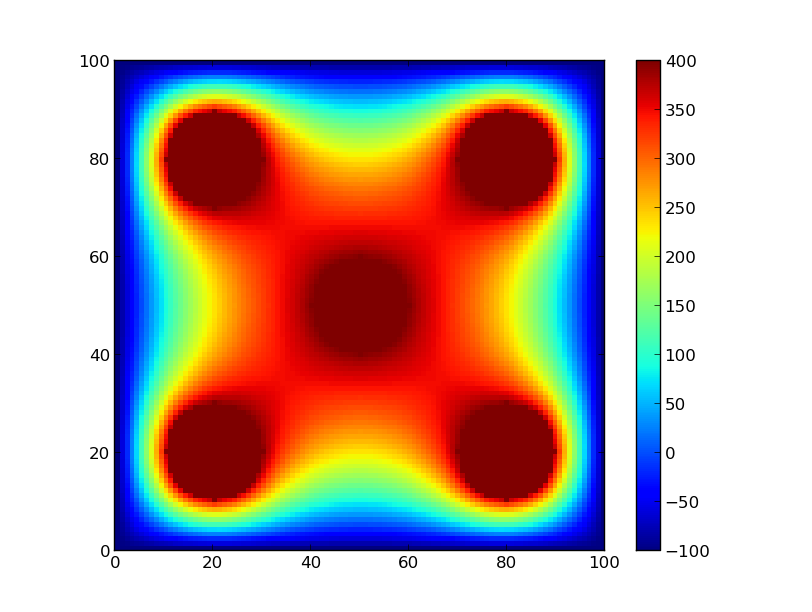
\includegraphics[scale=0.3]{imagenes/test5_gran1.png}
                \caption{Granularidad 1}
        \end{center}
\endminipage\hfill
\minipage{0.5\textwidth}
\begin{center}
        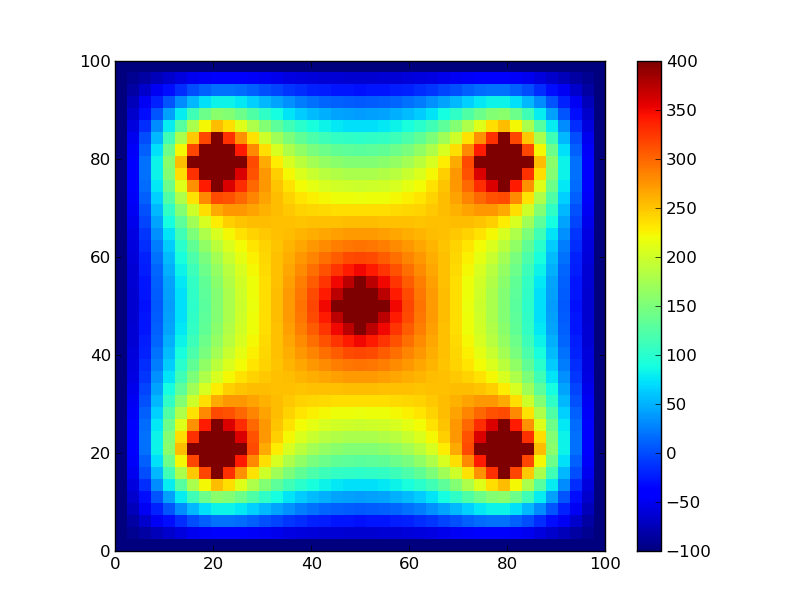
\includegraphics[scale=0.3]{imagenes/test5.png}
                \caption{Granularidad 2.5}
        \end{center}
\endminipage\hfill 
\end{figure}

\begin{figure}[!htb]
\minipage{0.5\textwidth}
\begin{center}
    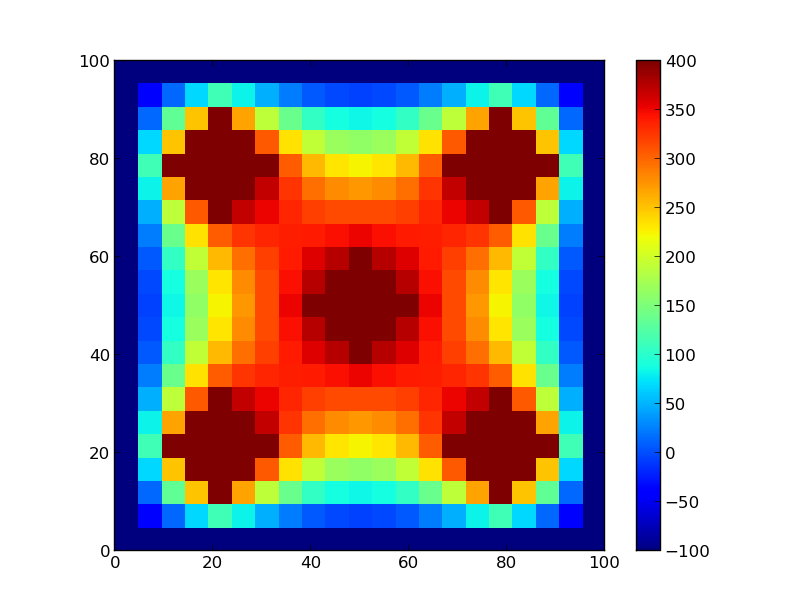
\includegraphics[scale=0.3]{imagenes/test5_gran5.png}
                \caption{Granularidad 5}
 \end{center}
\endminipage
\minipage{0.5\textwidth}
\begin{center}
   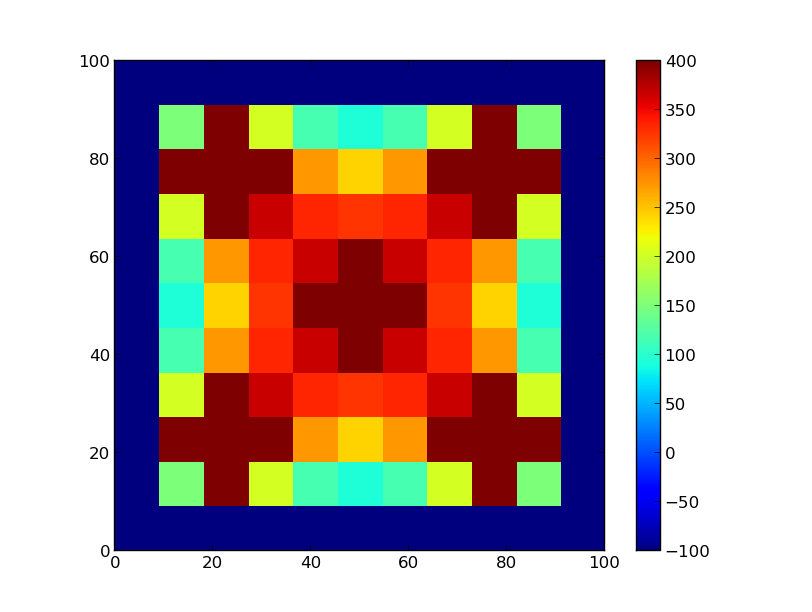
\includegraphics[scale=0.3]{imagenes/test5_gran10.png}
                \caption{Granularidad 10}
        \end{center}
\endminipage\hfill
\end{figure}
\clearpage

\subsubsection{Resultados Random}

A continuación observaremos un caso en la que la única sanguijuela que se debe eliminar es la del centro. Esta se encuentra exactamente en el punto central. Adicionalmente hay otras 4 sanguijuelas en las puntas. 
Matar a estas no soluciona nada ya que la del centro esta aplicando una temperatura constante de 400 Cº. Lo observaremos con 4 discretizaciones distintas para tener un mas amplio panorama.
\begin{figure}[htb]
\begin{center}
        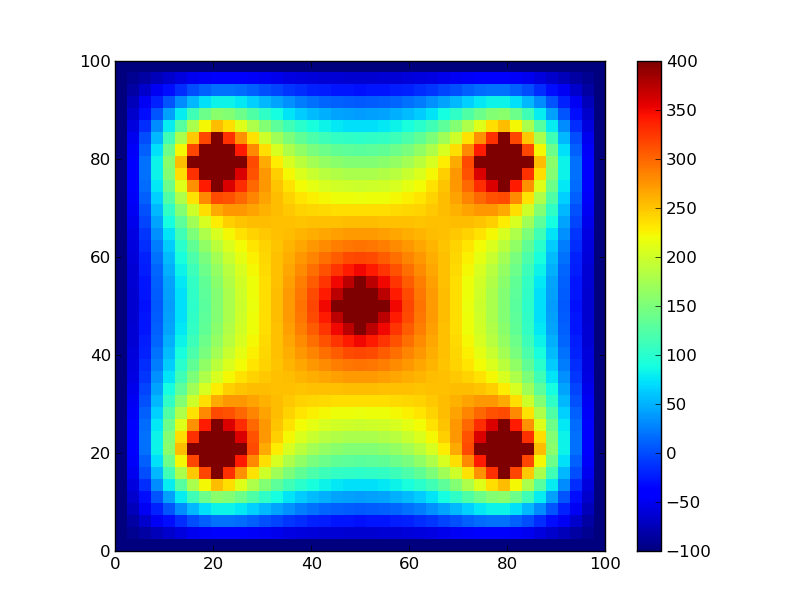
\includegraphics[scale=0.3]{imagenes/test5.png}
                \caption{Granularidad 2.5}
        \end{center}

\end{figure}

Ahora veamos que obtenemos al aplicarle distintas veces el algoritmo de solución random explicado en el desarrollo (\ref{sec:solucionRandom}).

\begin{figure}[htb]

\minipage{0.5\textwidth}
\begin{center}
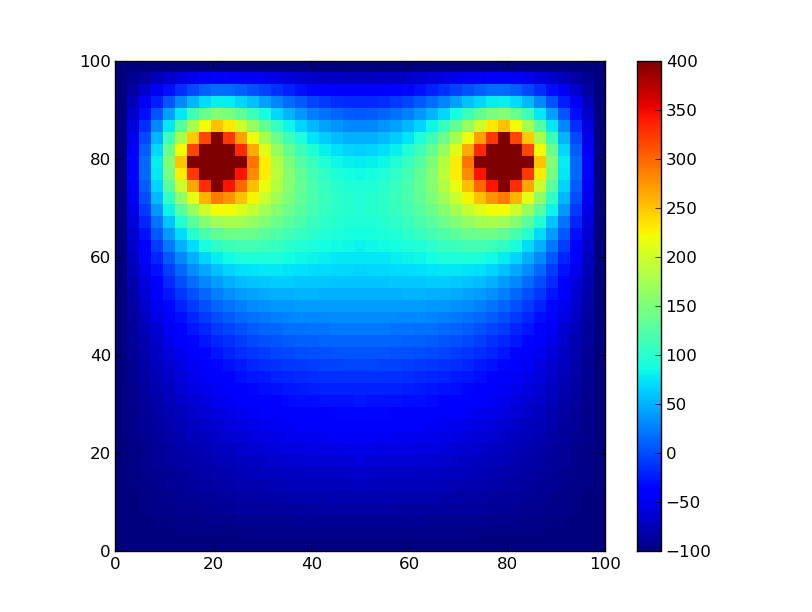
\includegraphics[scale=0.3]{imagenes/random_1.png} 
\caption{Resultado primer corrida} 
        \end{center}
\endminipage\hfill
\minipage{0.5\textwidth}
\begin{center}
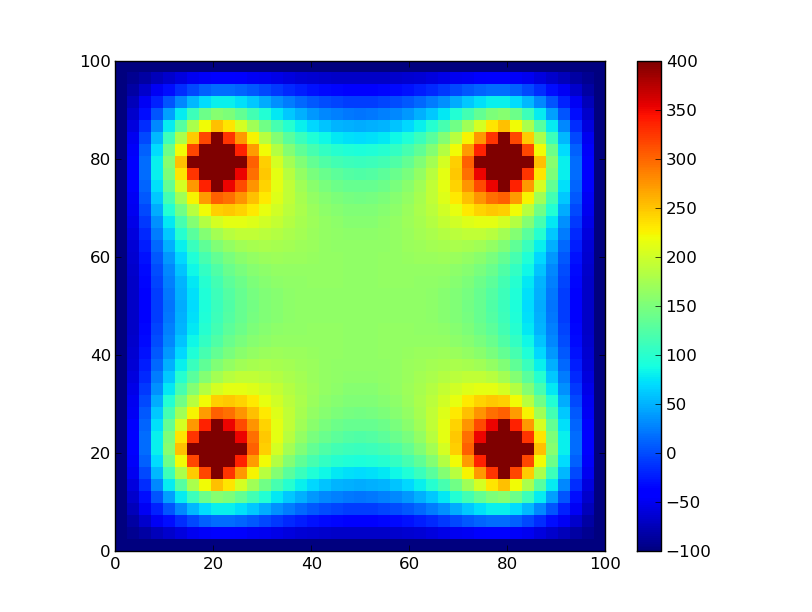
\includegraphics[scale=0.3]{imagenes/random_2.png} 
\caption{Resultado segunda corrida} 
        \end{center}
\endminipage\hfill 
\end{figure}

\begin{figure}[htb]
\begin{center}
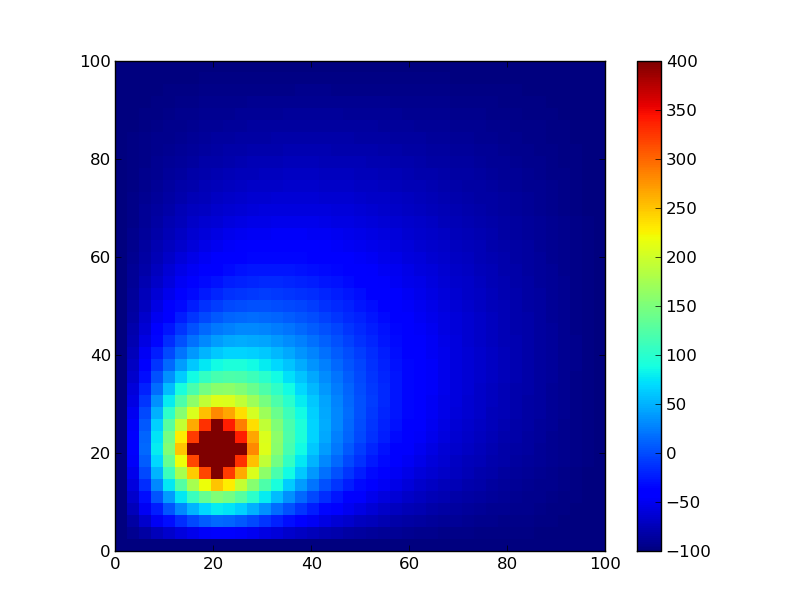
\includegraphics[scale=0.3]{imagenes/random_3.png} 
\caption{Resultado tercer corrida} 
\end{center}
\end{figure}
Como podemos observar la solución óptima (la que menos sanguijuelas elimina), es la segunda. Pero como esta solución es completamente random en la primera corrida mata 2 sanguijuelas antes de elegir 
la correcta y en la tercera 4. Sólo en la segunda elije en el primer intento la sanguijuela correcta. Se aplicó también para todas las granularidades antes mencionadas y se observó el mismo comportamiento erratico a la hora
de matar sanguijuelas. 

\clearpage


\subsubsection{Resultados Greedy}

Veamos ahora para la misma matriz como se comporta nuestro otro algoritmo. 


\begin{figure}[htb]
\begin{center}
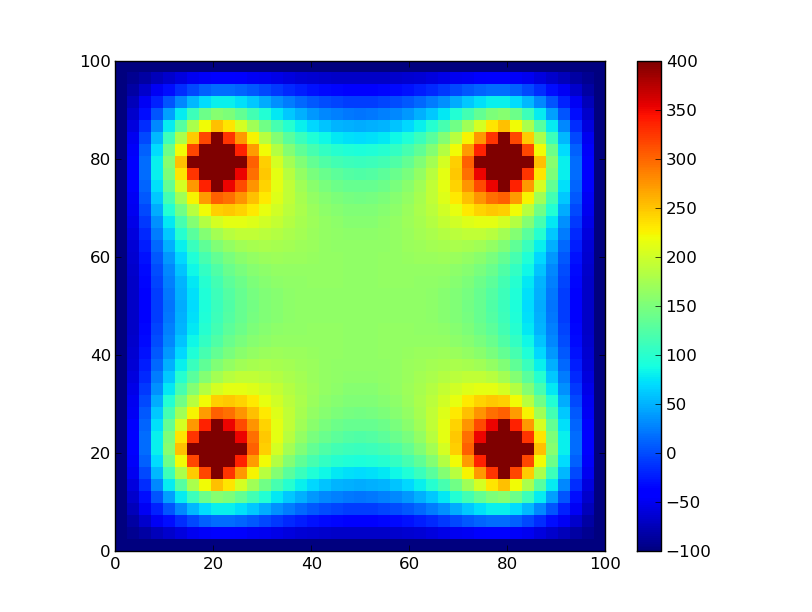
\includegraphics[scale=0.40]{imagenes/random_2.png} 
\caption{Resultado corrida con greedy} 
\end{center}
\end{figure}


En todas las corridas obtuvimos el mismo resultado y demoraron lo mismo. Era de esperarse, ya que efectivamente en este caso, la sanguijuela a eliminar era la del medio.
\newpage
\subsection{Resultados Banda VS Gaussiano}
Veamos ahora que realmente valió la pena la mejora al saber que era matriz banda en cuanto a tiempos en comparación con la eliminación gaussiana.
Anotamos que agregar un análisis de resultados no vale la pena ya que son el mismo

\begin{figure}[htb]
\begin{center}
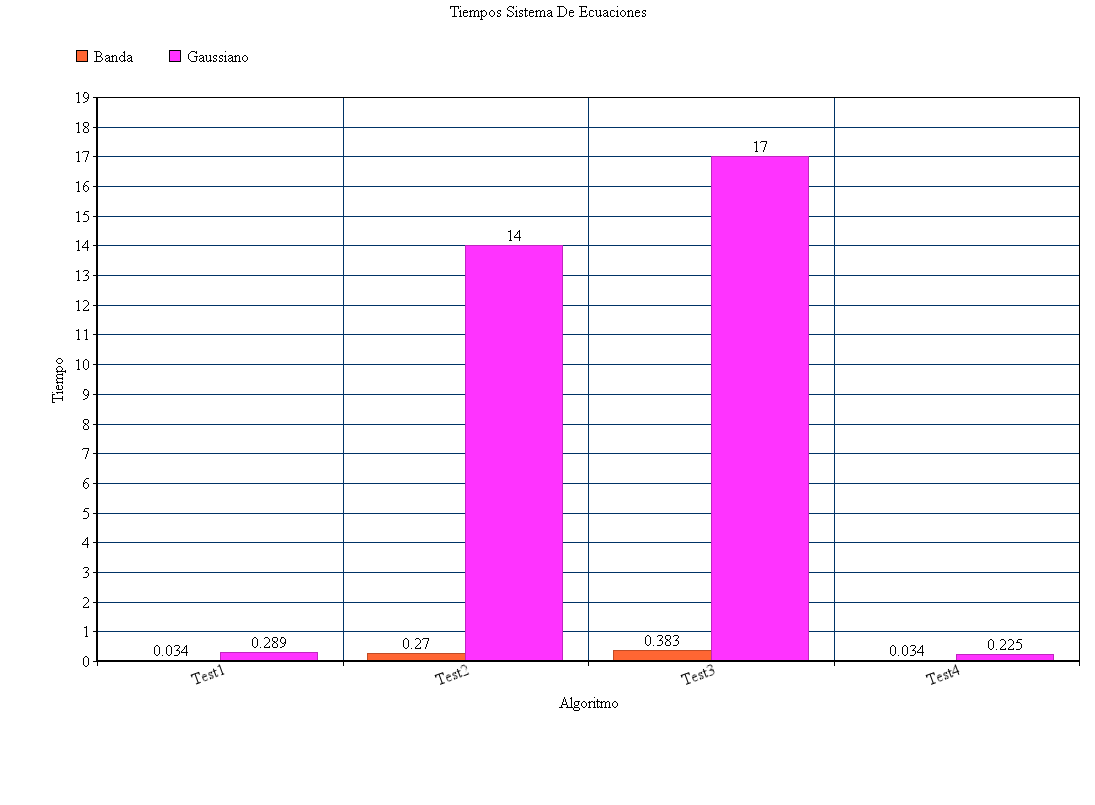
\includegraphics[scale=0.50]{imagenes/tiemposGaussVsBanda.png} 
\caption{Gauss VS Banda} 
\end{center}
\end{figure}
\clearpage
\subsection{Caso solución no es el mas cercano}

A continuación analizaremos un caso en el cual se debe eliminar una sanguijuela que no es la más cercana para efectivamente poder reducir la temperatura en punto crítico.
\begin{figure}[htb]
\begin{center}
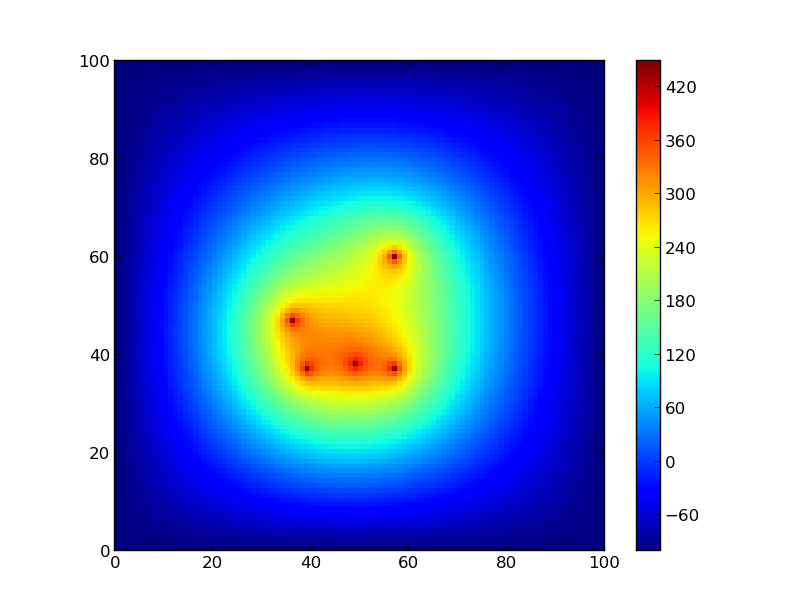
\includegraphics[scale=0.40]{imagenes/test6.png} 
\caption{Parabrisas granularidad 1} 
\end{center}
\end{figure}

Como podemos observar en las imágenes que están debajo, la solución greedy no es la óptima ya que mató a una sanguijuela extra. Esto es debido a que la principal radiación de calor era producida por el conjunto de 
sanguijuelas que están debajo del punto crítico y no por la mas cercana. Si eliminamos la sanguijuela central de aquel conjunto la radiación de calor emitida por él disminuye drásticamente en el punto crítico produciendo 
que la temperatura esté por debajo de los 235 grados sin necesidad de eliminar a las mas cercana. 

\begin{figure}[htb]
\minipage{0.5\textwidth}
\begin{center}
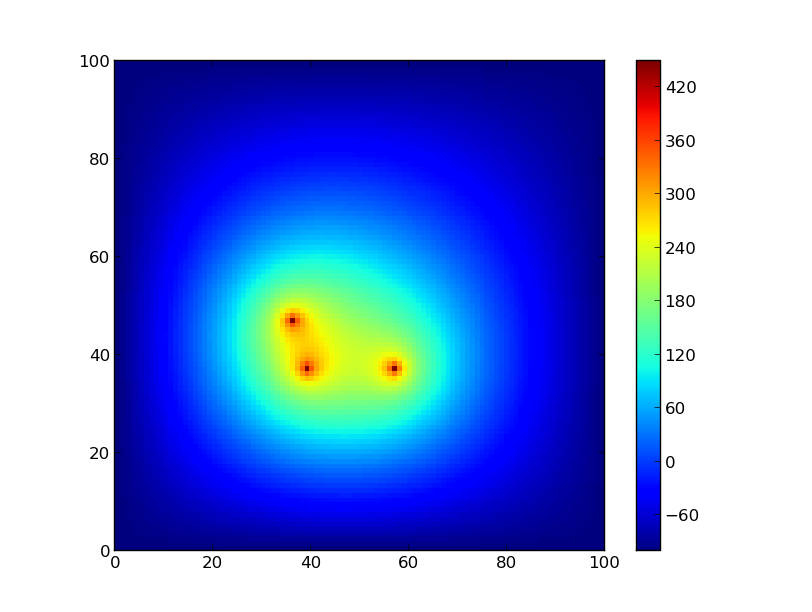
\includegraphics[scale=0.40]{imagenes/test6_greedy.png} 
\caption{Solución Greedy} 

        \end{center}
\endminipage\hfill
\minipage{0.5\textwidth}
\begin{center}
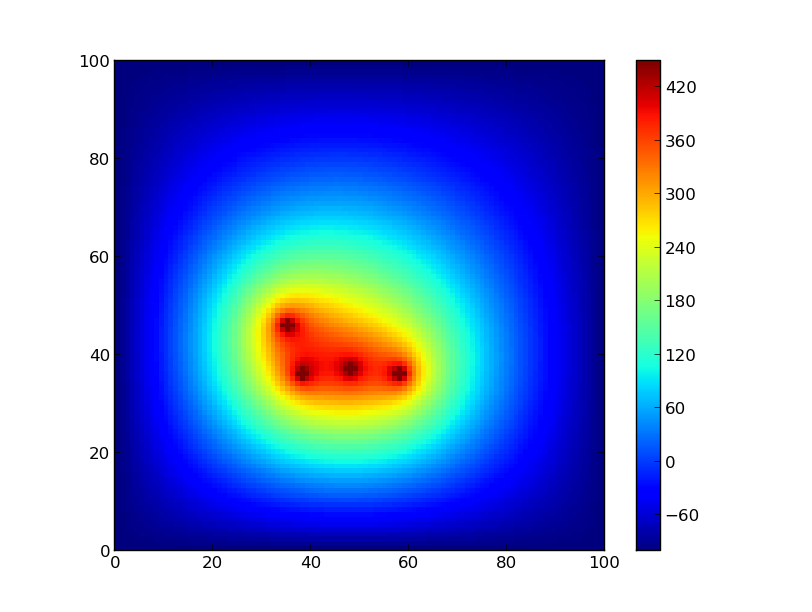
\includegraphics[scale=0.40]{imagenes/test6_solucion_real.png} 
\caption{Solución real} 
        \end{center}
\endminipage\hfill 


\end{figure}

Los datos exactos de este test son:

Medidas: 100 x 100 \\* 
discretización:1 \\* 
radio: 0.9 \\* 
tempreratura sanguijuelas:450 \\* 
Posiciónes sanguijuelas:\\* 
49 38\\* 
57 60\\* 
57 37\\* 
39 37\\* 
36 47 \\* 

El greedy mató primero a la sanguijuela de la posición (49,38) ya que era la mas cercana. Sin embargo si mataba primero la (57,60) la temperatura en el punto crítico disminuía lo suficiente. Esto pudimos corroborarlo al correr el test nuevamente sin esta última sangijuela y comprobando que tanto el greedy como random no mataban ninguna sangijuela ya que el punto crítica estaba por debajo de 235 grados celcius.

\subsubsection{Variando la granularidad}

Como vimos anteriormente, la temperatura en el punto crítico varía según la granularidad que le demos. Veamos entonces que pasa si aumentamos la granularidad (0.8 en vez de 1).

\begin{figure}[htb]
\minipage{0.5\textwidth}
\begin{center}
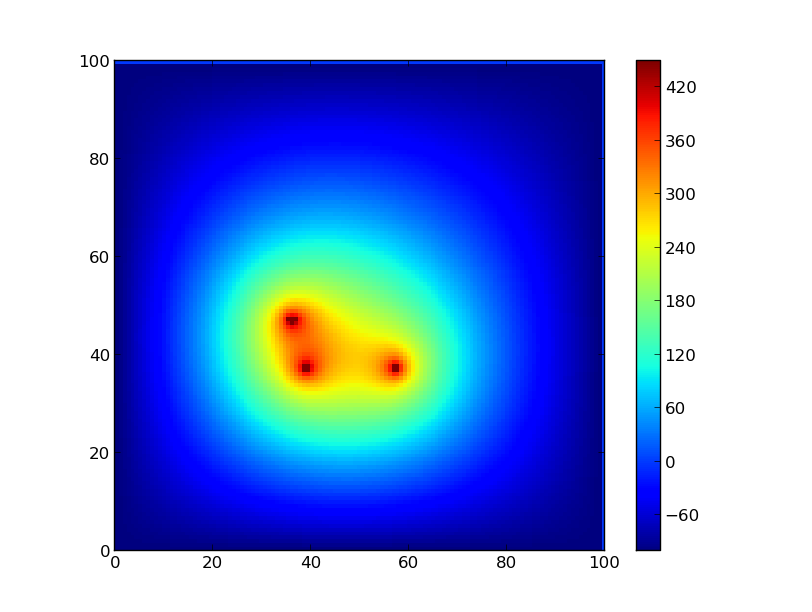
\includegraphics[scale=0.40]{imagenes/test6_g08_greedy.png} 
\caption{Solución Greedy} 

        \end{center}
\endminipage\hfill
\minipage{0.5\textwidth}
\begin{center}
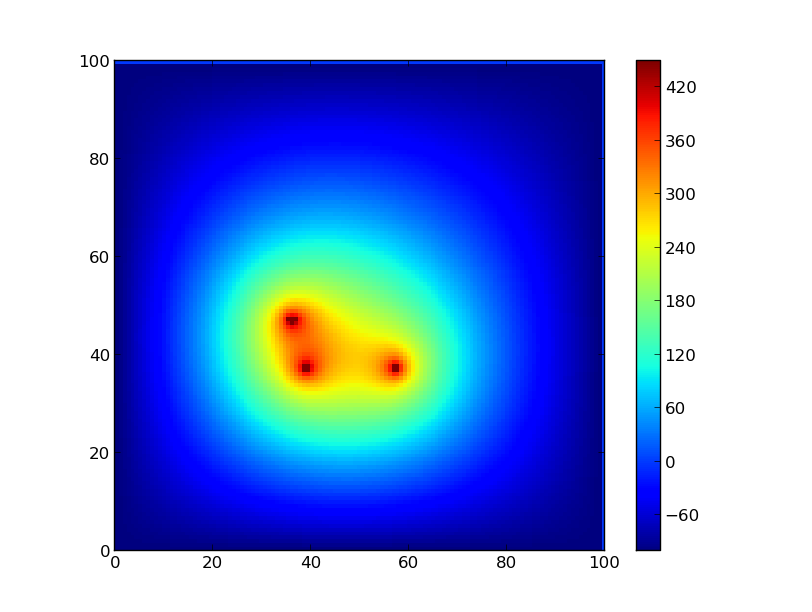
\includegraphics[scale=0.40]{imagenes/test6_g08_real.png} 
\caption{Solución real} 
        \end{center}
\endminipage\hfill 
\end{figure}

Como le aumentamos la granularidad aumentó la temperatura del punto central de tal forma que provocó que tampoco bastase eliminando una sola sangijuela, obteniendo así la misma cantidad de sangijuelas tanto en al solución real como en la greedy.

\newpage
\section{Discusi\'on}


\subsection{¿Por que random?}

Cuando empezamos a pensar otras soluciones alternativas a la golosa. Pensamos primero en soluciones totalmente suboptimas, como ir sacando desde el borde hacia el centro. Pero considerabamos que era tan malo que quitaba cualquier tipo de anàlisis serio. Luego también pensamos en ir sacando una del centro y una del borde alternadamente, pero no tenía tampoco algún justificativo conceptual alguno. Ahí fué entonces cuando pensamos en la solución random. Que claramente no responde a ningún compartamiento definido. Nos resultó mejor esto ya que las otras opciones pensadas o directamente estaban mal propuestas a proposito o no tenían sentido alguno. Además este comportamiento erratico podría llegar a darnos resultados interesantes o que rompiensen con nuestras intuiciones.









\newpage
\section{Conclusiones}

\subsection{Normal vs Banda}

De acuerdo a la experimentación realizada y a los resultados obtenidos no cabe duda que para resolver el problema planteado la mejor solución es utilizar el algoritmo de matriz banda. Principalmente porque los dos algoritmos proporcionan resultados iguales y exactos que resuelven el problema planteado, pero el algoritmo de banda los resuelve en tiempo y espacio extremadamente menor, y esta diferencia se diferencia aún mas a medida que aumenta el tamaño del parabrisas y aumenta la granularidad del mismo, hasta el punto en que al algoritmo normal deja de resolverlo en un tiempo razonable o excede la memoria provocando que se detenga el proceso que ejecuta. Por este motivo se concluye totalmente que el problema se debe solucionar mediante el algoritmo de banda.

\subsection{Random vs Greedy}

Como observamos en los resultados para el caso en el que la sanguijuela/s se encuentran en el medio claramente es mejor el greedy, ya que siempre mata a la sanguijuela correcta a diferencia del random que sólo lo hizo en uno de los 3 intentos. Por otro lado si tenemos en cuenta los tiempos que pueden llegar a demorar recalcular las temperaturas, esto le da todavía una mayor importancia, ya que se reduce considerablemente el tiempo de ejecución.

Por otro lado en el caso en el que la sanguijuela a sacar no era la más cercana, el random en promedio obtuvo mejores resultados. Sin embargo al aumentarle la granularidad esto se revertió nuevamente debido a que aumentó la temperatura del PC y esto provocó que si o si fuese necesario matar por lo menos dos sanguijuelas, entre ellas la mas cercana. \\
Lo que pensamos con respecto a esto es que hay casos bastantes puntuales en los que el greedy falla y el random podría devolver una mejor solución, aunque esto también depende del porcentaje de sanguijuelas que se puedan sacar para solucionar el problema. Es decir, si de 5 sanguijuelas por ejemplo la solución no está en sacar la mas cercana sino cualquiera de las otras 4, el random sería el mejor, pero si la correcta fuera una sola, el random volvería a ser tan o mas ineficiente que el greedy ya que tendría una probabilidad de 1/5 de elegir la correcta la primera vez.\\
Osea, el random se comportaría mejor que el greedy sólo en el caso de que la sanguijuela a sacar no sea la más cercana y haya otras n/2 (o más) posibles para sacar de forma que resuelvan el problema.

Finalmente concluimos que los casos en los que el random sería mejor que el greedy son tan puntuales y nuestro problema, en principio, es tan genérico que son despreciables. Por lo que el greedy termina siendo claramente mejor.







\newpage

\end{document}

